% gof_report.tex — Goodness-of-fit report for χ_eff spin population models
% Compile: pdflatex gof_report.tex (figures must be present in working dir)
\documentclass[11pt,a4paper]{article}

\usepackage[utf8]{inputenc}
\usepackage[T1]{fontenc}
\usepackage{amsmath,amssymb}
\usepackage{graphicx}
\usepackage{booktabs}
\usepackage[margin=2.5cm]{geometry}
\usepackage{hyperref}
\usepackage{natbib}
\usepackage{xspace}

% ── Shortcuts ────────────────────────────────────────────────────────────────
\newcommand{\chieff}{\ensuremath{\chi_\mathrm{eff}}\xspace}
\newcommand{\chisq}{\ensuremath{\chi^2}\xspace}
\newcommand{\Nev}{\ensuremath{N_\mathrm{ev}}\xspace}
\newcommand{\Nbin}{\ensuremath{N_\mathrm{bin}}\xspace}
\newcommand{\Nmock}{\ensuremath{N_\mathrm{mock}}\xspace}

\title{Calibrated Goodness-of-Fit Test for Effective-Spin Population Models}
\author{Automated Pipeline Report}
\date{\today}

\begin{document}
\maketitle

% ══════════════════════════════════════════════════════════════════════════════
\begin{abstract}
We apply a calibrated $\chi^2$ goodness-of-fit test to five population models
for the effective inspiral spin parameter \chieff of binary black-hole mergers
observed during the LIGO--Virgo--KAGRA O3 and O4 observing runs.  The test
compares binned distributions of the 5th- and 95th-percentile \chieff
posterior quantiles for \Nev~=~71 events against predictions from
re-weighted injection sets.  $p$-values are obtained by Monte Carlo
calibration under each model's own null hypothesis.  We report results for the
Isotropic, Azzalini skew-normal, LVK Default, Truncated Gaussian, and
Roulet+\,2021 three-component mixture models.
\end{abstract}

% ══════════════════════════════════════════════════════════════════════════════
\section{Method}\label{sec:method}

\subsection{Observable and binning}

For each event $i$ in the catalog we extract the 5th and 95th percentiles of
the marginal posterior on \chieff, denoted $q_i^{5}$ and $q_i^{95}$.  We
form a concatenated histogram vector
\begin{equation}
  \mathbf{h} = \bigl(\,h_1^{5},\dots,h_{\Nbin}^{5},\;
                      h_1^{95},\dots,h_{\Nbin}^{95}\bigr),
\end{equation}
where $\Nbin = 15$ equally spaced bins cover the range of observed quantiles
(with 10\% margin on each side).  Each sub-histogram is normalised to sum to
unity so that $\mathbf{h}$ has $2\Nbin = 30$ entries.

\subsection{Population models and injection re-weighting}

We consider five population models for the \chieff distribution:

\paragraph{Model 1: Isotropic spins.}
Component spins are uniform in magnitude on $[0,\chi_\mathrm{max}]$ and
isotropic in orientation. No free parameters; the injection prior itself
is the population.

\paragraph{Model 2: Azzalini skew-normal (scipy).}
The standard Azzalini skew-normal distribution~\citep{Azzalini1985},
as implemented in \texttt{scipy.stats.skewnorm}:
\begin{equation}
  p(\chieff \mid a,\xi,\omega) = \frac{2}{\omega}\,
  \phi\!\left(\frac{\chieff - \xi}{\omega}\right)\,
  \Phi\!\left(a\,\frac{\chieff - \xi}{\omega}\right),
\end{equation}
truncated to $[-1,1]$, where $\phi$ and $\Phi$ are the standard normal
PDF and CDF, $a$ is the shape (skewness), $\xi$ the location, and
$\omega$ the scale.
Best-fit: $(a,\xi,\omega) = (13.44, -0.069, 0.161)$.
\emph{Note:} This is \textbf{not} the LVK epsilon-skew-normal
(split-normal) parameterisation.

\paragraph{Model 3: LVK Default.}
Spin magnitudes follow truncated normals on $[0,1]$:
\begin{equation}
  p(\chi_i \mid \mu_\chi,\sigma_\chi) = \mathcal{N}_T(\chi_i;\,\mu_\chi,\sigma_\chi,\,0,1),
  \qquad i \in \{1,2\}.
\end{equation}
Tilt angles are a mixture of an aligned and an isotropic component:
\begin{equation}
  p(\cos\theta_1,\cos\theta_2 \mid \mu_t,\sigma_t,\zeta)
  = \zeta\,\prod_{i=1}^{2}\mathcal{N}_T(\cos\theta_i;\,\mu_t,\sigma_t,\,-1,1)
  + \frac{1-\zeta}{4}.
\end{equation}
Five free parameters: $(\mu_\chi,\sigma_\chi,\mu_t,\sigma_t,\zeta)$.
MAP from GWTC-4.0: $(0.091, 0.318, 0.752, 0.884, 0.382)$.

\paragraph{Model 4: Truncated Gaussian.}
\begin{equation}
  p(\chieff \mid \mu,\sigma) = \mathcal{N}_T(\chieff;\,\mu,\sigma,\,-1,1).
\end{equation}
Median from GWTC-4.0: $(\mu,\sigma) = (0.042, 0.103)$.

\paragraph{Model 5: Three-component mixture \citep[Roulet+\,2021]{Roulet2021}.}
Three half-Gaussians centered at $\chieff = 0$:
\begin{equation}
  p(\chieff \mid \zeta_+,\zeta_-,\sigma)
  = \zeta_0\,\mathcal{N}_T(\chieff;\,0,\sigma_0,\,-1,1)
  + \zeta_-\,\mathcal{N}_T(\chieff;\,0,\sigma,\,-1,0)
  + \zeta_+\,\mathcal{N}_T(\chieff;\,0,\sigma,\,0,1),
\end{equation}
where $\zeta_0 = 1 - \zeta_+ - \zeta_-$ and $\sigma_0 = 0.04$ (fixed).
The first component is a narrow ``nonspinning'' peak; the second and third
are anti-aligned and aligned half-Gaussians with shared width $\sigma$.
MLE from O1--O3a: $(\zeta_+, \zeta_-, \sigma) = (0.45, 0.00, 0.23)$.
The data are consistent with no anti-aligned component ($\zeta_- = 0$).

Figure~\ref{fig:ppds} shows the intrinsic $\chieff$ probability density
for each model at its best-fit hyperparameters, without selection effects.

\begin{figure}[htbp]
  \centering
  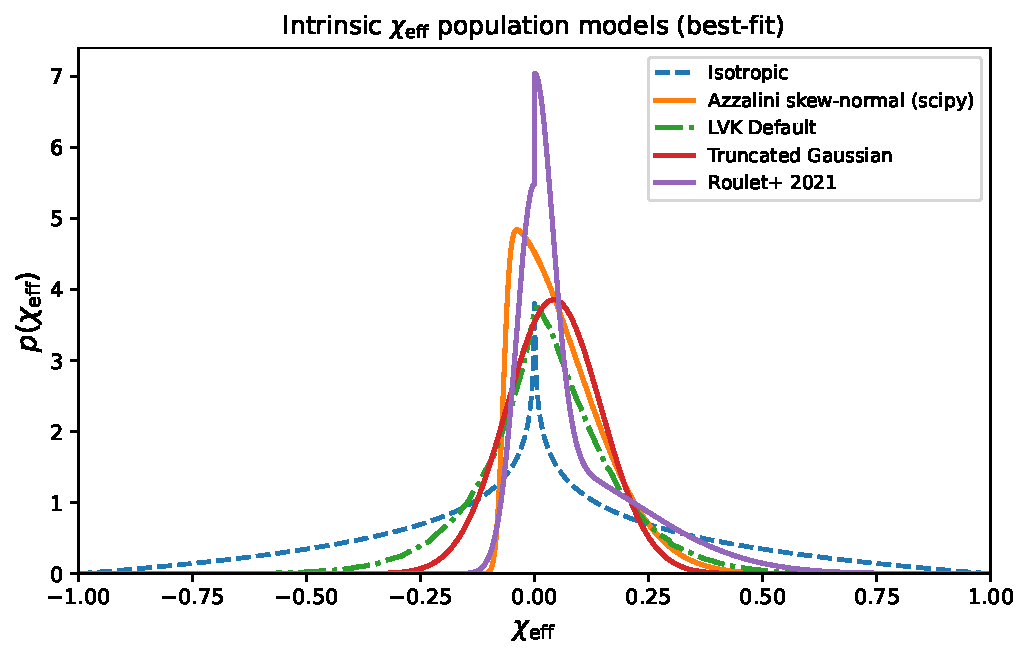
\includegraphics[width=0.85\textwidth]{fig_intrinsic_ppds.pdf}
  \caption{Intrinsic $\chieff$ population distributions at the best-fit
           hyperparameters for each model (no selection effects applied).
           The isotropic model is broad and symmetric, while the
           skew-normal, truncated Gaussian, and two-Gaussian mixture all
           peak sharply near $\chieff \approx 0.1$.  The LVK Default
           model, which operates in component-spin space, produces a
           broader $\chieff$ distribution peaked near zero.}
  \label{fig:ppds}
\end{figure}

Each model defines per-injection importance weights
$w_k(\boldsymbol{\theta})$ that re-weight the found-injection set from its
astrophysical prior to the target population.  The predicted histogram
$\mathbf{h}^\mathrm{pred}$ is obtained by building the same binned
representation from the weighted injections.

\subsection{$\chi^2$ test statistic}

\subsection{$\chi^2$ test statistic}

For a given set of hyperparameters $\boldsymbol{\theta}$, each injection $k$
receives an importance weight
$w_k(\boldsymbol{\theta}) = p_\mathrm{pop}(\chi_{\mathrm{eff},k};\boldsymbol{\theta})
\,/\, p_\mathrm{prior}(\chi_{\mathrm{eff},k}, q_k)$,
where $p_\mathrm{prior}$ is the isotropic-spin prior of the injection campaign
(evaluated analytically following Callister et al.).
To estimate the predicted histogram $\boldsymbol{\mu}(\boldsymbol{\theta})$
and its covariance $\hat{\Sigma}(\boldsymbol{\theta})$,
we draw $B = 1000$ bootstrap catalogues of \Nev events from the injection set
with sampling probabilities $\propto w_k(\boldsymbol{\theta})$, histogram
each, and compute the sample mean and covariance of the resulting histogram
vectors.  Bins with zero bootstrap variance (never populated) are projected
out before inversion.

The test statistic is then
\begin{equation}\label{eq:chi2}
  \chi^2(\boldsymbol{\theta})
  = \bigl(\mathbf{h}^\mathrm{obs} - \boldsymbol{\mu}(\boldsymbol{\theta})\bigr)^T
    \,\hat{\Sigma}(\boldsymbol{\theta})^{+}\,
    \bigl(\mathbf{h}^\mathrm{obs} - \boldsymbol{\mu}(\boldsymbol{\theta})\bigr),
\end{equation}
where $\hat{\Sigma}^{+}$ denotes the Moore--Penrose pseudoinverse.

\subsection{Calibrated $p$-values}

Each population model comes with a set of best-fit hyperparameters
$\boldsymbol{\theta}_\mathrm{BF}$ obtained from hierarchical Bayesian
inference on the same event catalogue (see Table~\ref{tab:results} for
sources).  We wish to test: \emph{is} $\boldsymbol{\theta}_\mathrm{BF}$
\emph{consistent with the observed catalogue?}

A complication is that $\boldsymbol{\theta}_\mathrm{BF}$ was itself inferred
from the data.  To account for this, we allow the test statistic to be
minimised over $\boldsymbol{\theta}$:
\begin{equation}\label{eq:chi2min}
  \chi^2_\mathrm{min} = \min_{\boldsymbol{\theta}}\;
  \chi^2(\boldsymbol{\theta}),
\end{equation}
using the Nelder--Mead simplex algorithm (3 random restarts from
$\boldsymbol{\theta}_\mathrm{BF}$ and two random points in the prior
volume), yielding the best-fit parameters
$\hat{\boldsymbol{\theta}} = \arg\min_{\boldsymbol{\theta}}\,
\chi^2(\boldsymbol{\theta})$.
For models with no free parameters (Isotropic),
$\hat{\boldsymbol{\theta}} = \boldsymbol{\theta}_\mathrm{BF}$.

To calibrate the $p$-value we ask: if the true population were
$\boldsymbol{\theta}_\mathrm{BF}$, how often would a catalogue of \Nev
events yield a $\chi^2_\mathrm{min}$ as large as observed?
\begin{enumerate}
  \item Generate mock catalogue~$j$ by drawing \Nev events from the
        injection set with probabilities
        $\propto w_k(\boldsymbol{\theta}_\mathrm{BF})$.
  \item Beings in mock universe~$j$ do not know
        $\boldsymbol{\theta}_\mathrm{BF}$.  They minimise
        $\chi^2(\boldsymbol{\theta})$ on their own catalogue, obtaining
        $\chi^2_{\mathrm{min},j}$.
  \item Repeat for $j = 1, \dots, \Nmock$.
\end{enumerate}
The calibrated $p$-value is
\begin{equation}
  p = \frac{1}{\Nmock}
      \sum_{j=1}^{\Nmock}
      \mathbb{1}\!\bigl[\chi^2_{\mathrm{min},j}
      \ge \chi^2_\mathrm{min,\,obs}\bigr].
\end{equation}
This construction accounts for the ``look-elsewhere effect'' of fitting:
because each mock catalogue is also fitted, the null distribution of
$\chi^2_\mathrm{min}$ is shifted to lower values relative to the
fixed-$\boldsymbol{\theta}$ distribution, and the resulting $p$-value is
appropriately conservative.

% ══════════════════════════════════════════════════════════════════════════════
\section{Results}\label{sec:results}

Table~\ref{tab:results} summarises the goodness-of-fit results for each
model.  Figures~\ref{fig:pvalues}--\ref{fig:null} show the $p$-value
comparison, example histogram overlay, and null distribution, respectively.

% ── Results table ────────────────────────────────────────────────────────────
% Full 5-model results (500 mocks)
\begin{table}[htbp]
\centering
\caption{Calibrated goodness-of-fit results for \Nev~=~71 events,
$\Nbin = 15$ bins per quantile (30 histogram entries total),
bin edges set to the observed quantile range $\pm 10\%$ margin.
$N_\mathrm{params}$ is the number of free parameters;
$N_\mathrm{eff}$ is the effective injection sample size after
re-weighting; $\chi^2_\mathrm{min} = \chi^2(\hat{\boldsymbol{\theta}})$ is the test statistic at
the best-fit $\hat{\boldsymbol{\theta}}$; $p$ is the Monte Carlo calibrated $p$-value
(\Nmock~=~500).}
\label{tab:results}
\begin{tabular}{lccccp{4.5cm}}
\toprule
Model & $N_\mathrm{params}$ & $N_\mathrm{eff}$ & $\chi^2_\mathrm{min}$ & $p$-value &
  $\boldsymbol{\theta}_\mathrm{BF}$ \\
\midrule
Isotropic          & 0 & 8728  & 41.02 & 0.074 & --- \\
Skew-normal        & 3 & 4696  & 9.21  & 0.548 & $a{=}13.44$, $\xi{=}{-}0.069$, $\omega{=}0.161$ \\
LVK Default        & 5 & 3296  & 20.05 & 0.146 & $\mu_\chi{=}0.091$, $\sigma_\chi{=}0.318$, $\mu_t{=}0.752$, $\sigma_t{=}0.884$, $\zeta{=}0.382$ \\
Truncated Gaussian & 2 & 5006  & 15.69 & 0.230 & $\mu{=}0.042$, $\sigma{=}0.103$ \\
Roulet+ 2021       & 3 & 4444  & 13.72 & 0.258 & $\zeta_+{=}0.45$, $\zeta_-{=}0.00$, $\sigma{=}0.23$ \\
\end{tabular}
\end{table}

% ── Figures ──────────────────────────────────────────────────────────────────
\begin{figure}[htbp]
  \centering
  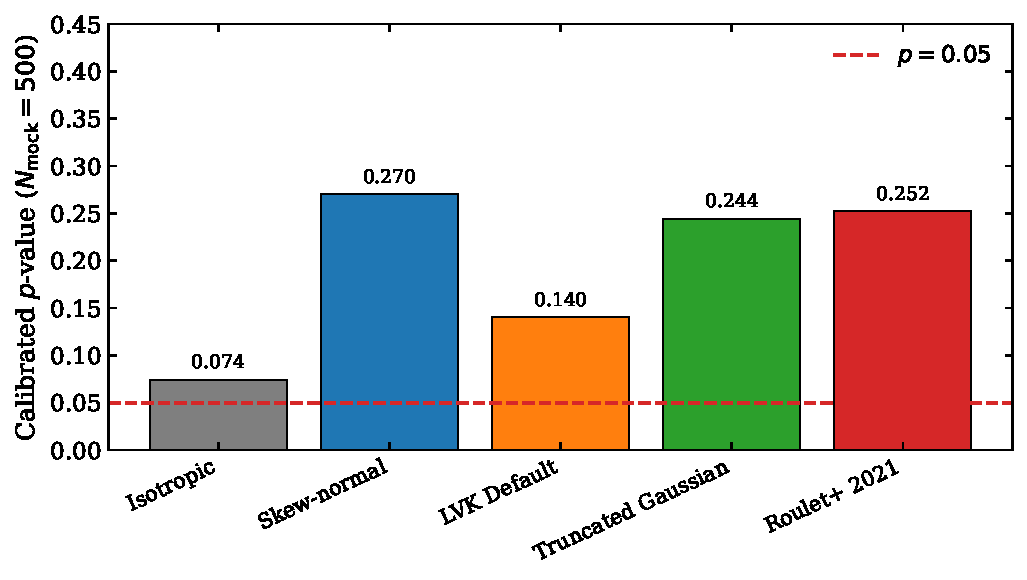
\includegraphics[width=0.85\textwidth]{fig_pvalues_summary.pdf}
  \caption{Summary of calibrated $p$-values for all five \chieff population
           models.}
  \label{fig:pvalues}
\end{figure}

\begin{figure}[htbp]
  \centering
  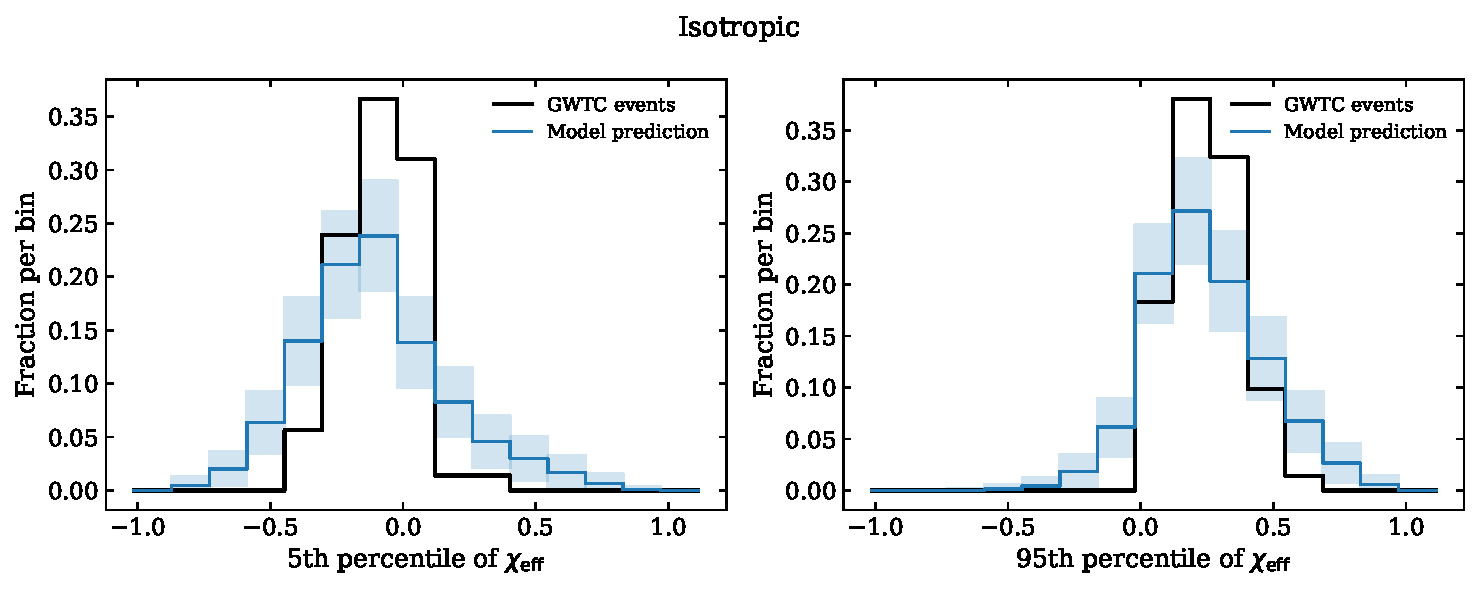
\includegraphics[width=0.48\textwidth]{fig_hist_isotropic.pdf}\hfill
  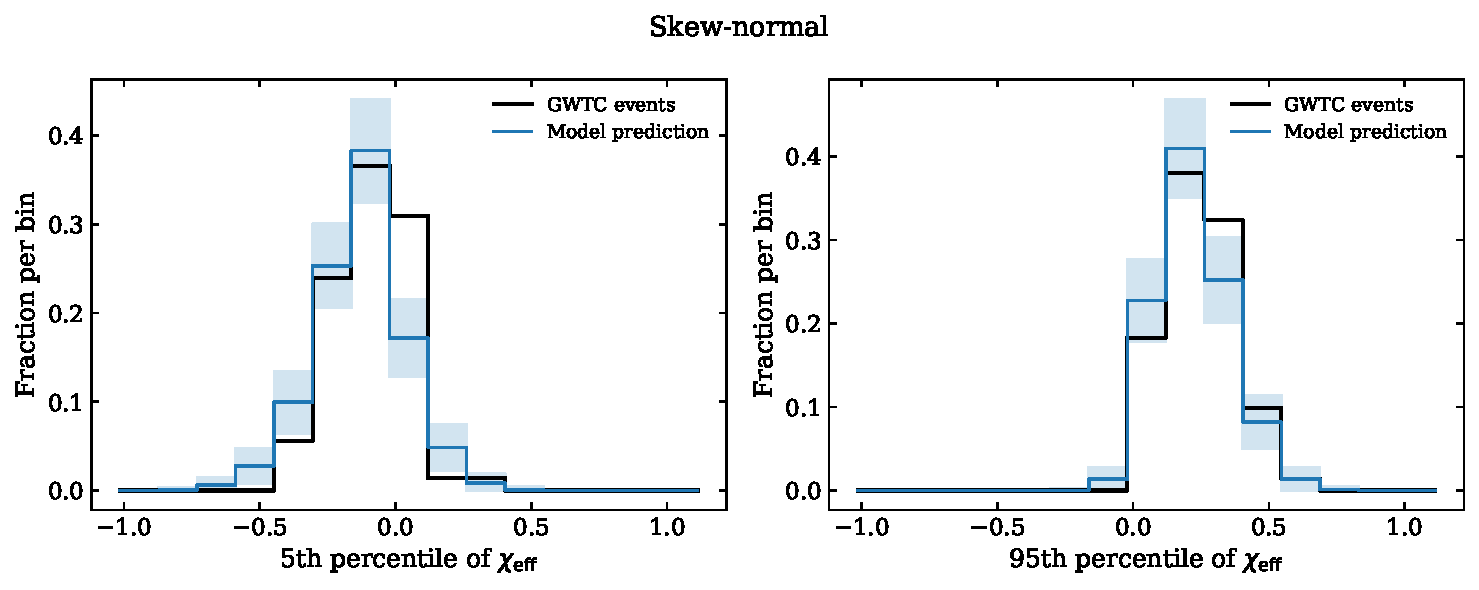
\includegraphics[width=0.48\textwidth]{fig_hist_skewnorm.pdf}\\[6pt]
  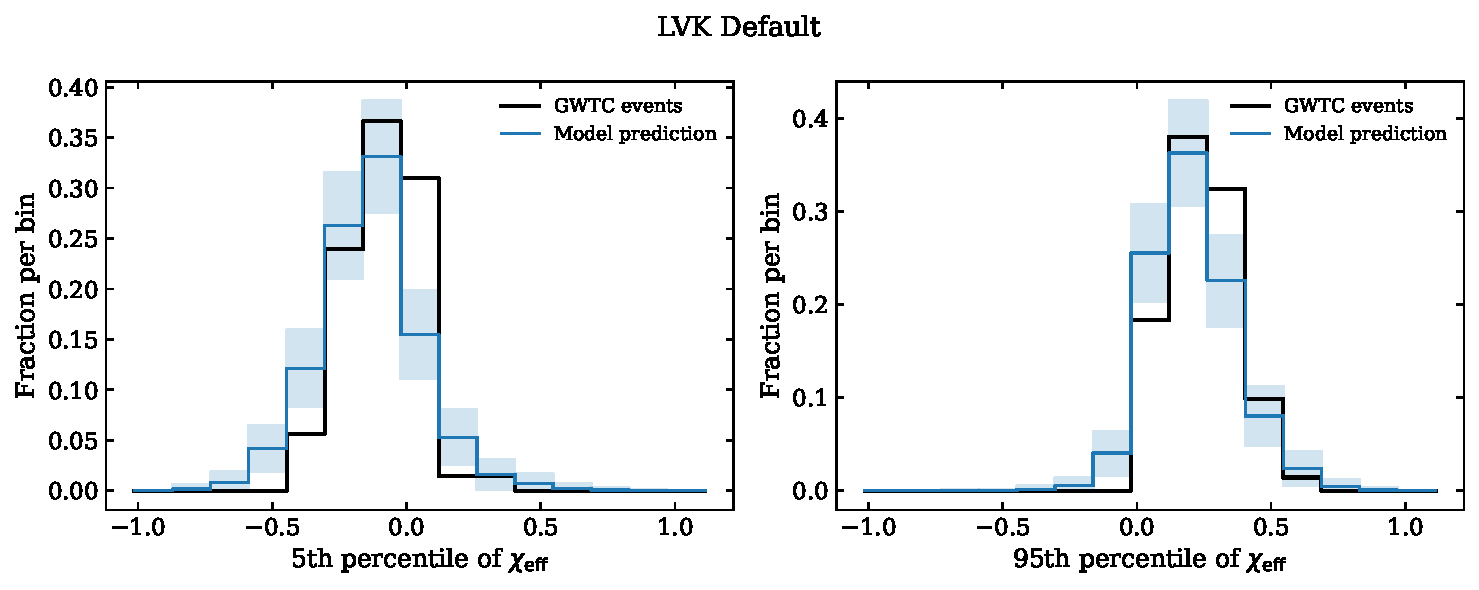
\includegraphics[width=0.48\textwidth]{fig_hist_lvk.pdf}\hfill
  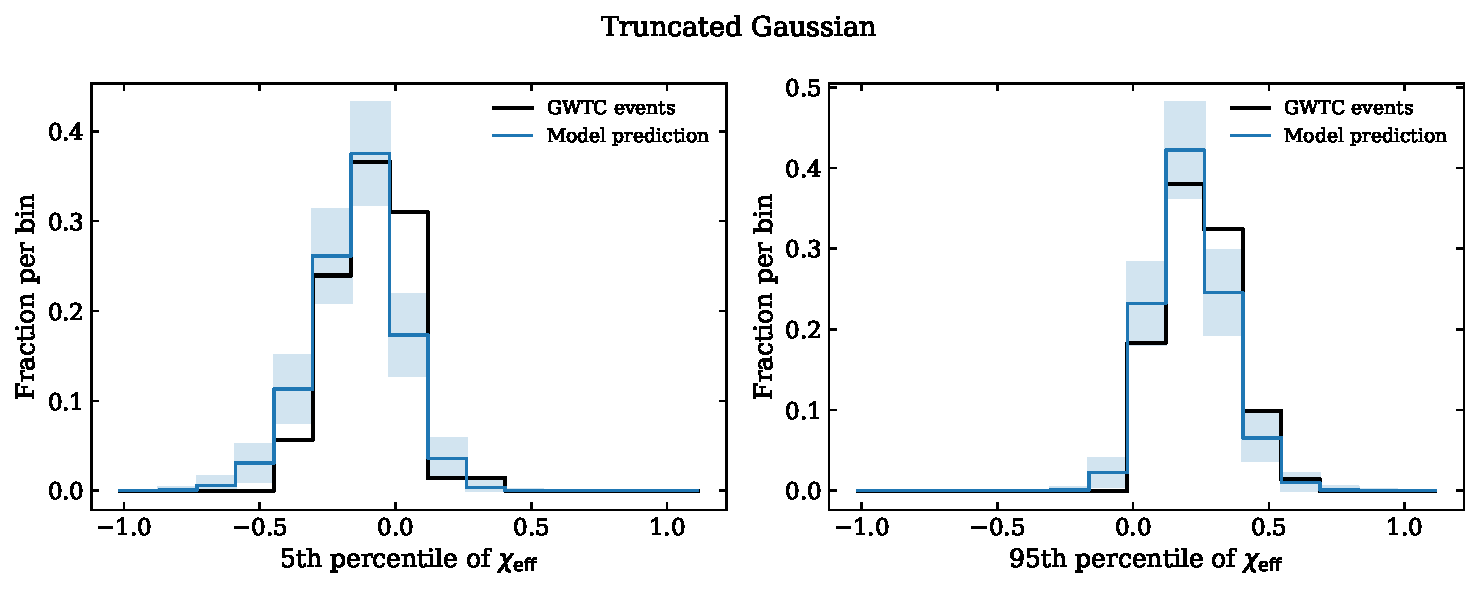
\includegraphics[width=0.48\textwidth]{fig_hist_truncgauss.pdf}\\[6pt]
  \centering
  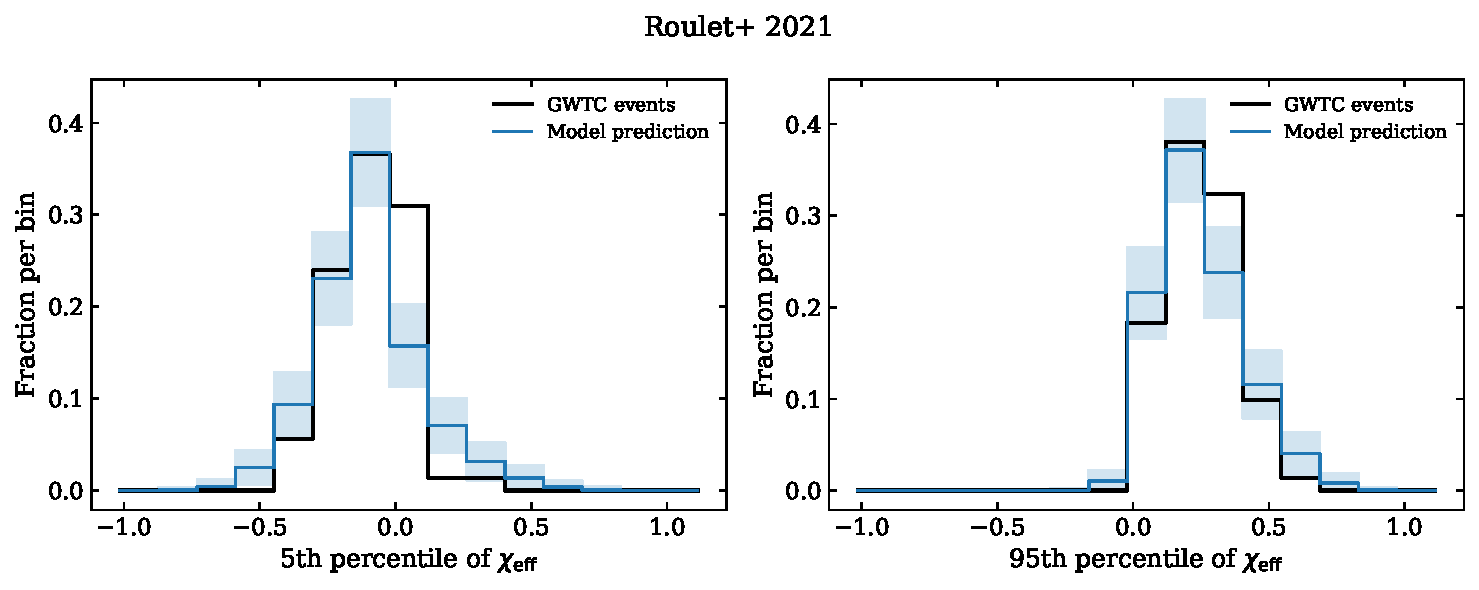
\includegraphics[width=0.48\textwidth]{fig_hist_roulet.pdf}
  \caption{Histogram overlays of observed (data) vs.\ predicted (model)
           quantile distributions for all five models.  The model
           prediction and $1\sigma$ bootstrap band are evaluated at
           $\hat{\boldsymbol{\theta}}$.}
  \label{fig:hist}
\end{figure}

\begin{figure}[htbp]
  \centering
  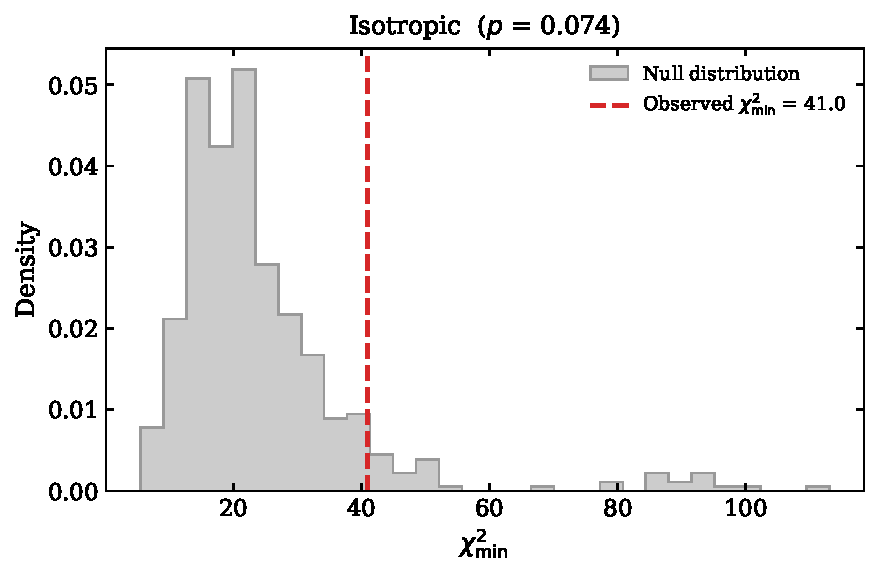
\includegraphics[width=0.48\textwidth]{fig_null_isotropic.pdf}\hfill
  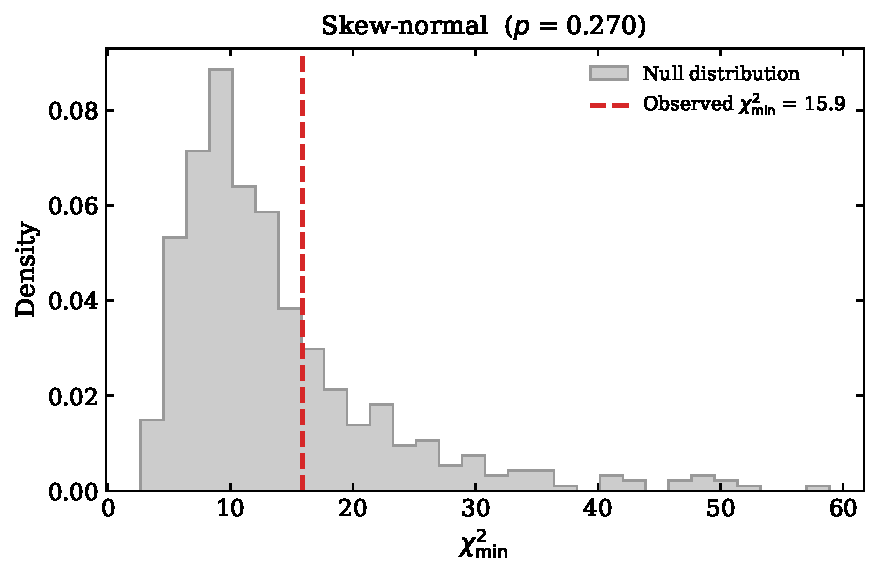
\includegraphics[width=0.48\textwidth]{fig_null_skewnorm.pdf}\\[6pt]
  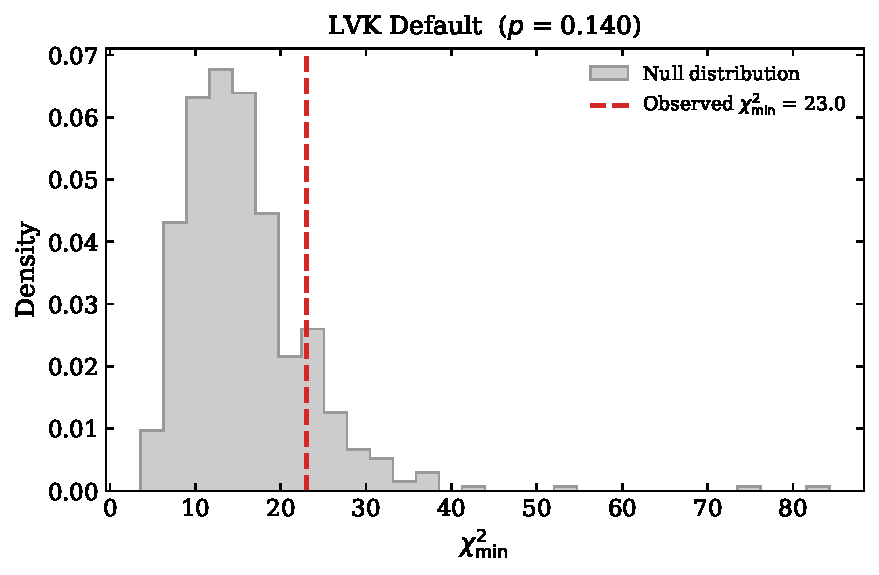
\includegraphics[width=0.48\textwidth]{fig_null_lvk.pdf}\hfill
  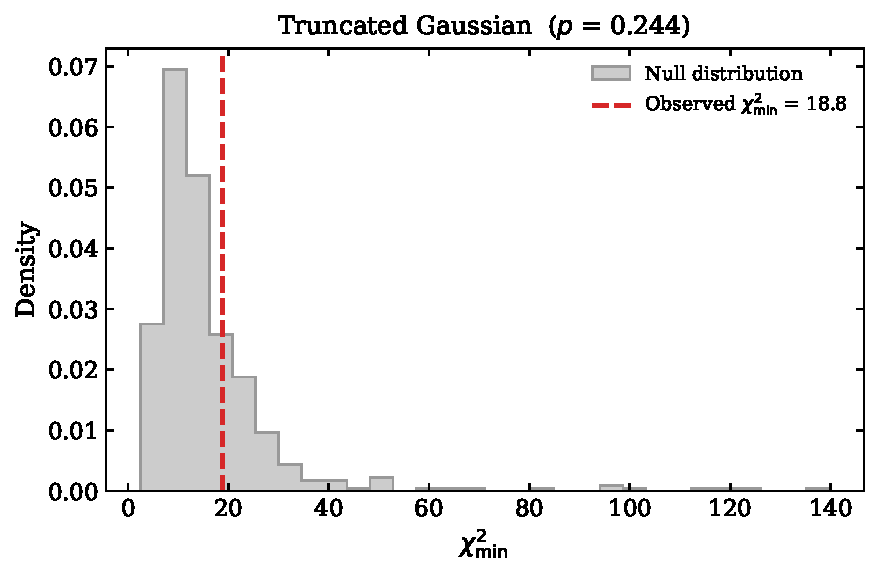
\includegraphics[width=0.48\textwidth]{fig_null_truncgauss.pdf}\\[6pt]
  \centering
  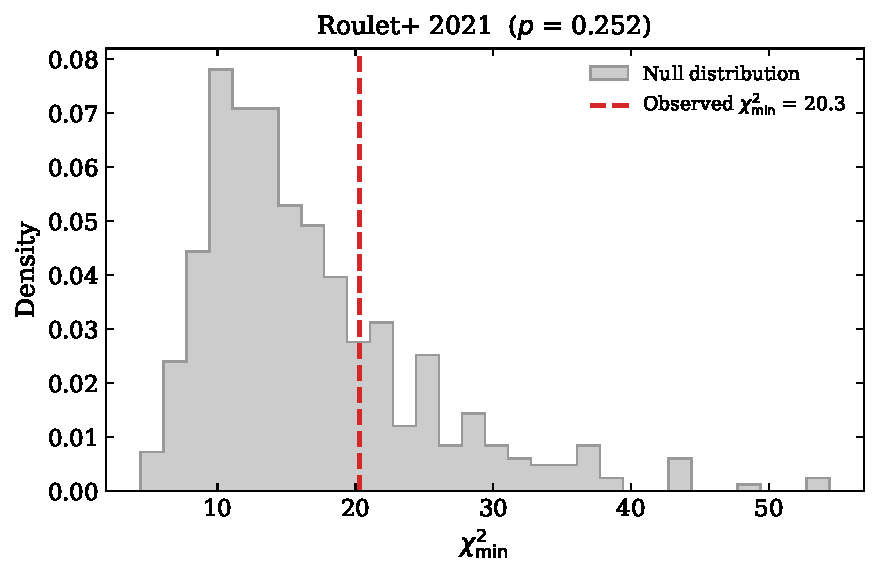
\includegraphics[width=0.48\textwidth]{fig_null_roulet.pdf}
  \caption{Null distributions of $\chi^2_\mathrm{min}$ from \Nmock~=~500
           mock catalogues for all five models.  The vertical dashed line
           marks the observed $\chi^2_\mathrm{min}$.}
\end{figure}

% ══════════════════════════════════════════════════════════════════════════════
\section{Binning-free diagnostic: CDF comparison}\label{sec:cdf}

The $\chi^2$ test statistic depends on the choice of histogram binning.
We find that $p$-values change appreciably when the number of bins is
varied (e.g.\ from $\Nbin = 10$ to 15), because the covariance matrix
is sensitive to the number of empty or near-empty bins.

As a complementary, binning-free diagnostic, we compare the empirical
cumulative distribution functions (CDFs) of the observed and predicted
$\chieff$ quantiles.  For a given $\boldsymbol{\theta}$, the model CDF
is the importance-weighted empirical CDF of the injection quantiles:
\begin{equation}
  F_\mathrm{model}(x \mid \boldsymbol{\theta})
  = \frac{\sum_{k:\,q_k \le x} w_k(\boldsymbol{\theta})}
         {\sum_k w_k(\boldsymbol{\theta})}.
\end{equation}
The test statistic is the two-sample Kolmogorov--Smirnov distance
between the observed and model CDFs, summed over both quantiles:
\begin{equation}\label{eq:ks}
  D(\boldsymbol{\theta})
  = \sup_x \bigl|F_\mathrm{obs}^{5}(x) - F_\mathrm{model}^{5}(x)\bigr|
  + \sup_x \bigl|F_\mathrm{obs}^{95}(x) - F_\mathrm{model}^{95}(x)\bigr|.
\end{equation}
This is evaluated without any binning and requires only sorting
($\sim 1$~ms per evaluation, compared to $\sim 100$~ms for the
bootstrap-based $\chi^2$).

The calibrated $p$-value follows the same logic as in
Section~\ref{sec:method}: minimise $D(\boldsymbol{\theta})$ for the
real catalogue (Nelder--Mead, 3 restarts), generate mock catalogues from
$\boldsymbol{\theta}_\mathrm{BF}$, let each mock minimise
$D(\boldsymbol{\theta})$, and compute
$p = \Nmock^{-1}\sum_j \mathbb{1}[D_{\mathrm{min},j} \ge D_\mathrm{min,obs}]$.

Figures~\ref{fig:cdf5} and~\ref{fig:cdf95} show the empirical CDF
comparison for the 5th and 95th percentiles, respectively.
The model CDF and bootstrap band are evaluated at
$\hat{\boldsymbol{\theta}}_\mathrm{KS}$ (the KS-minimised parameters
from Table~\ref{tab:ks}).

\paragraph{Parameter shifts under minimisation.}
An important diagnostic is whether $\hat{\boldsymbol{\theta}}$ moves
significantly from $\boldsymbol{\theta}_\mathrm{BF}$ during
minimisation.  Table~\ref{tab:shifts} compares the two for the $\chi^2$
and KS statistics.  The $\chi^2$ optimiser moves modestly from
$\boldsymbol{\theta}_\mathrm{BF}$ for most models.  The KS optimiser
moves further, particularly for the LVK Default model where the tilt
parameters shift substantially ($\sigma_t: 0.88 \to 0.13$, $\zeta:
0.38 \to 0.77$).  Large shifts indicate that the hierarchical best-fit
$\boldsymbol{\theta}_\mathrm{BF}$ does not minimise the GoF statistic,
i.e.\ the population model at its published parameters is not the
best-fitting member of the model family for this observable.

\begin{table}[htbp]
\centering
\caption{Best-fit parameters $\hat{\boldsymbol{\theta}}$ from $\chi^2$
and KS minimisation, compared to $\boldsymbol{\theta}_\mathrm{BF}$ from
hierarchical inference.  Only models with free parameters are shown.
$^\dagger$Nelder--Mead exited the physical parameter bounds
($\zeta_+ > 1$); result invalid and being recomputed with
bounded optimisation.}
\label{tab:shifts}
\small
\begin{tabular}{lp{3.8cm}p{3.8cm}p{3.8cm}}
\toprule
Model & $\boldsymbol{\theta}_\mathrm{BF}$ & $\hat{\boldsymbol{\theta}}_{\chi^2}$ & $\hat{\boldsymbol{\theta}}_\mathrm{KS}$ \\
\midrule
Skew-normal & $(13.44, -0.069, 0.161)$ & $(16.40, -0.041, 0.174)$ & $(8.89, 0.011, 0.123)$ \\
LVK Default & $(0.091, 0.318, 0.752, 0.884, 0.382)$ & $(0.091, 0.318, 0.752, 0.884, 0.382)$ & $(0.110, 0.277, 0.457, 0.131, 0.774)$ \\
Trunc.\ Gauss. & $(0.042, 0.103)$ & $(0.045, 0.103)$ & $(0.105, 0.080)$ \\
Roulet+ & $(0.45, 0.00, 0.23)$ & $(0.50, 0.00, 0.18)$ & invalid$^\dagger$ \\
\bottomrule
\end{tabular}
\end{table}

\begin{figure}[htbp]
  \centering
  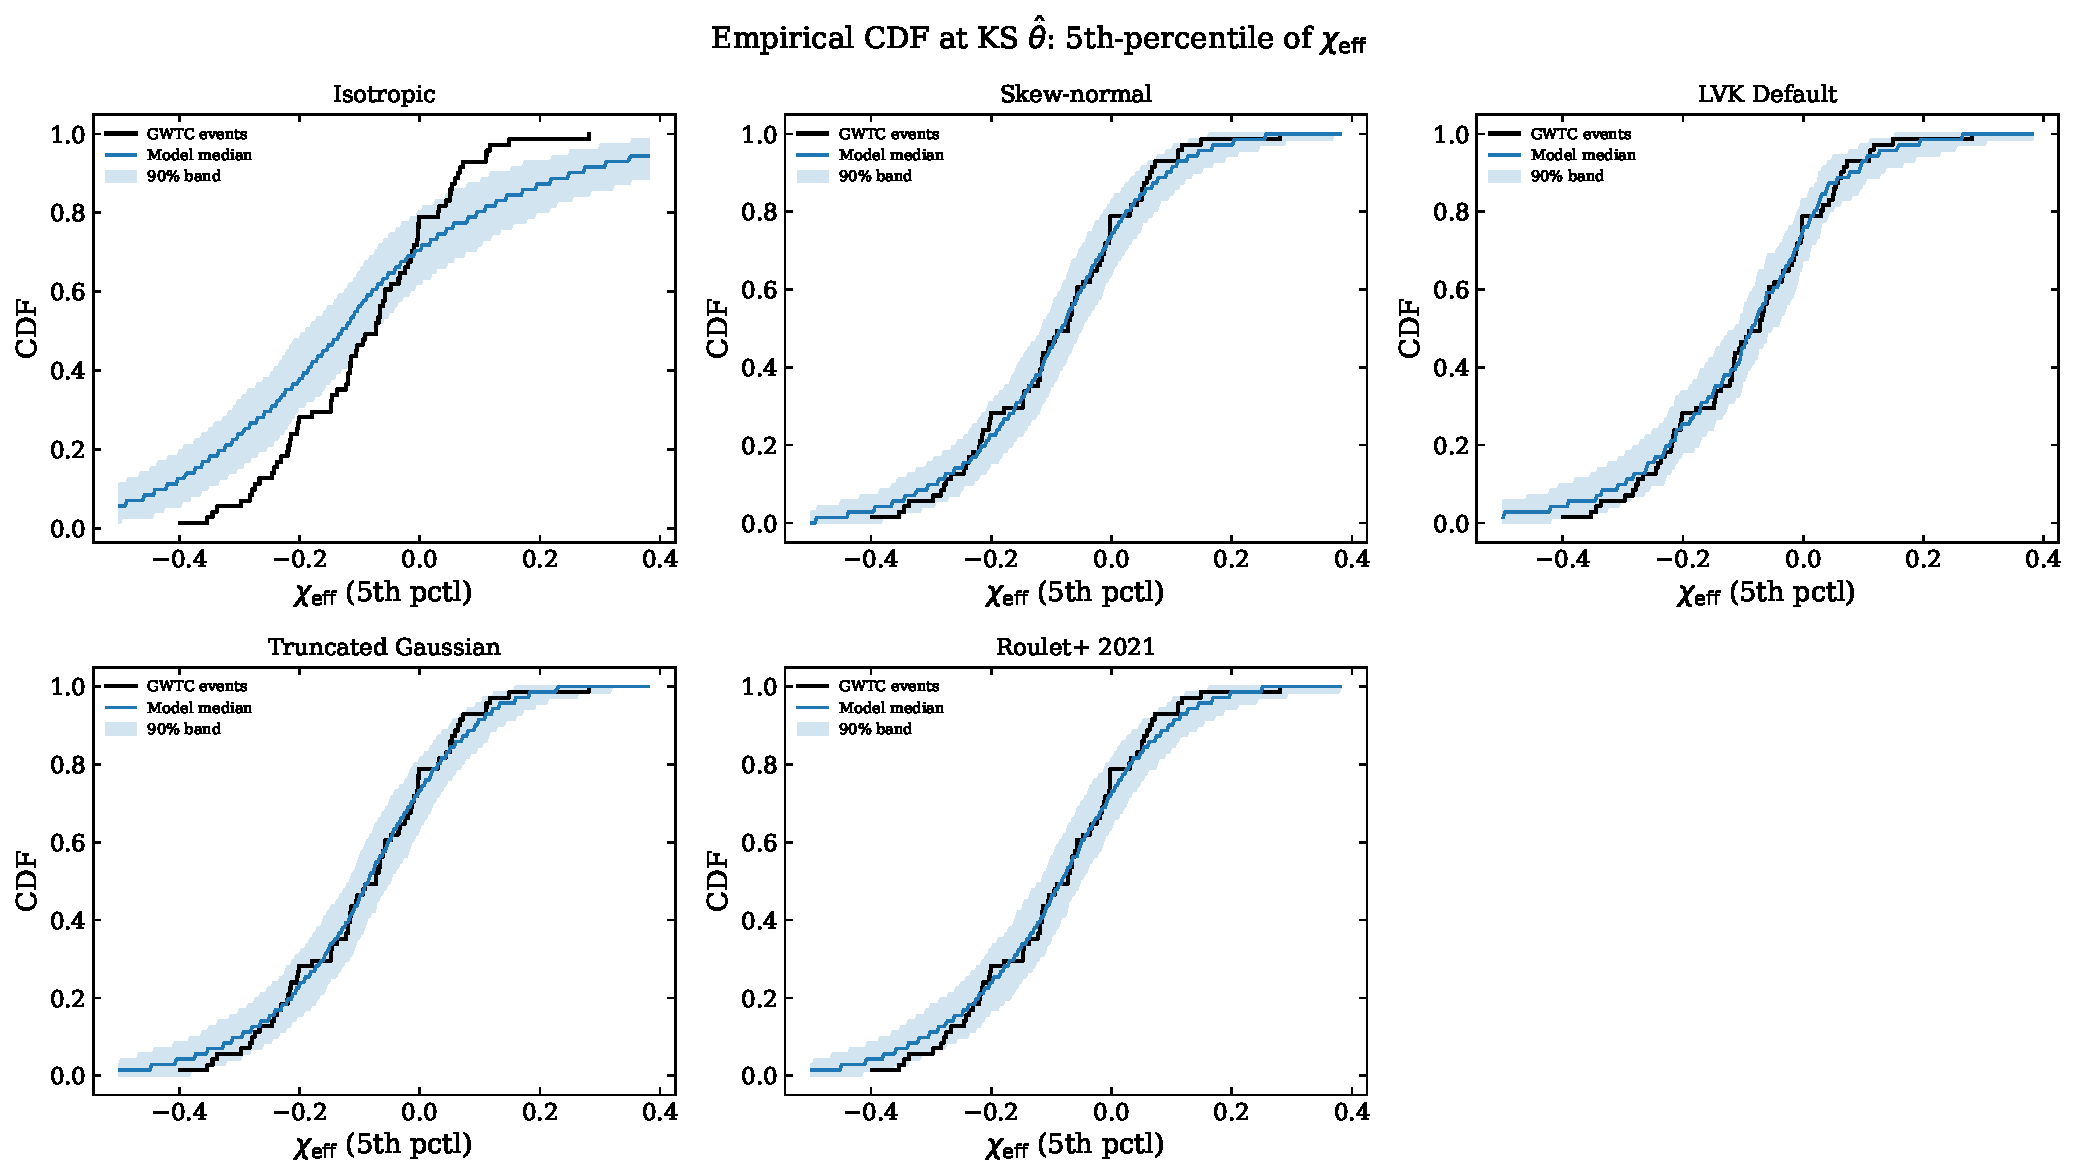
\includegraphics[width=\textwidth]{fig_cdf_5th.pdf}
  \caption{Empirical CDF comparison for the 5th percentile of \chieff.
           Black step function: observed events (71 steps).
           Blue curve: median model CDF at
           $\hat{\boldsymbol{\theta}}_\mathrm{KS}$.  Blue band: 90\% envelope
           from 500 bootstrap draws of 71 events from the model,
           showing the expected scatter from finite catalogue size.
           Where the black curve exits the band, the model is in
           tension with the data.}
  \label{fig:cdf5}
\end{figure}

\begin{figure}[htbp]
  \centering
  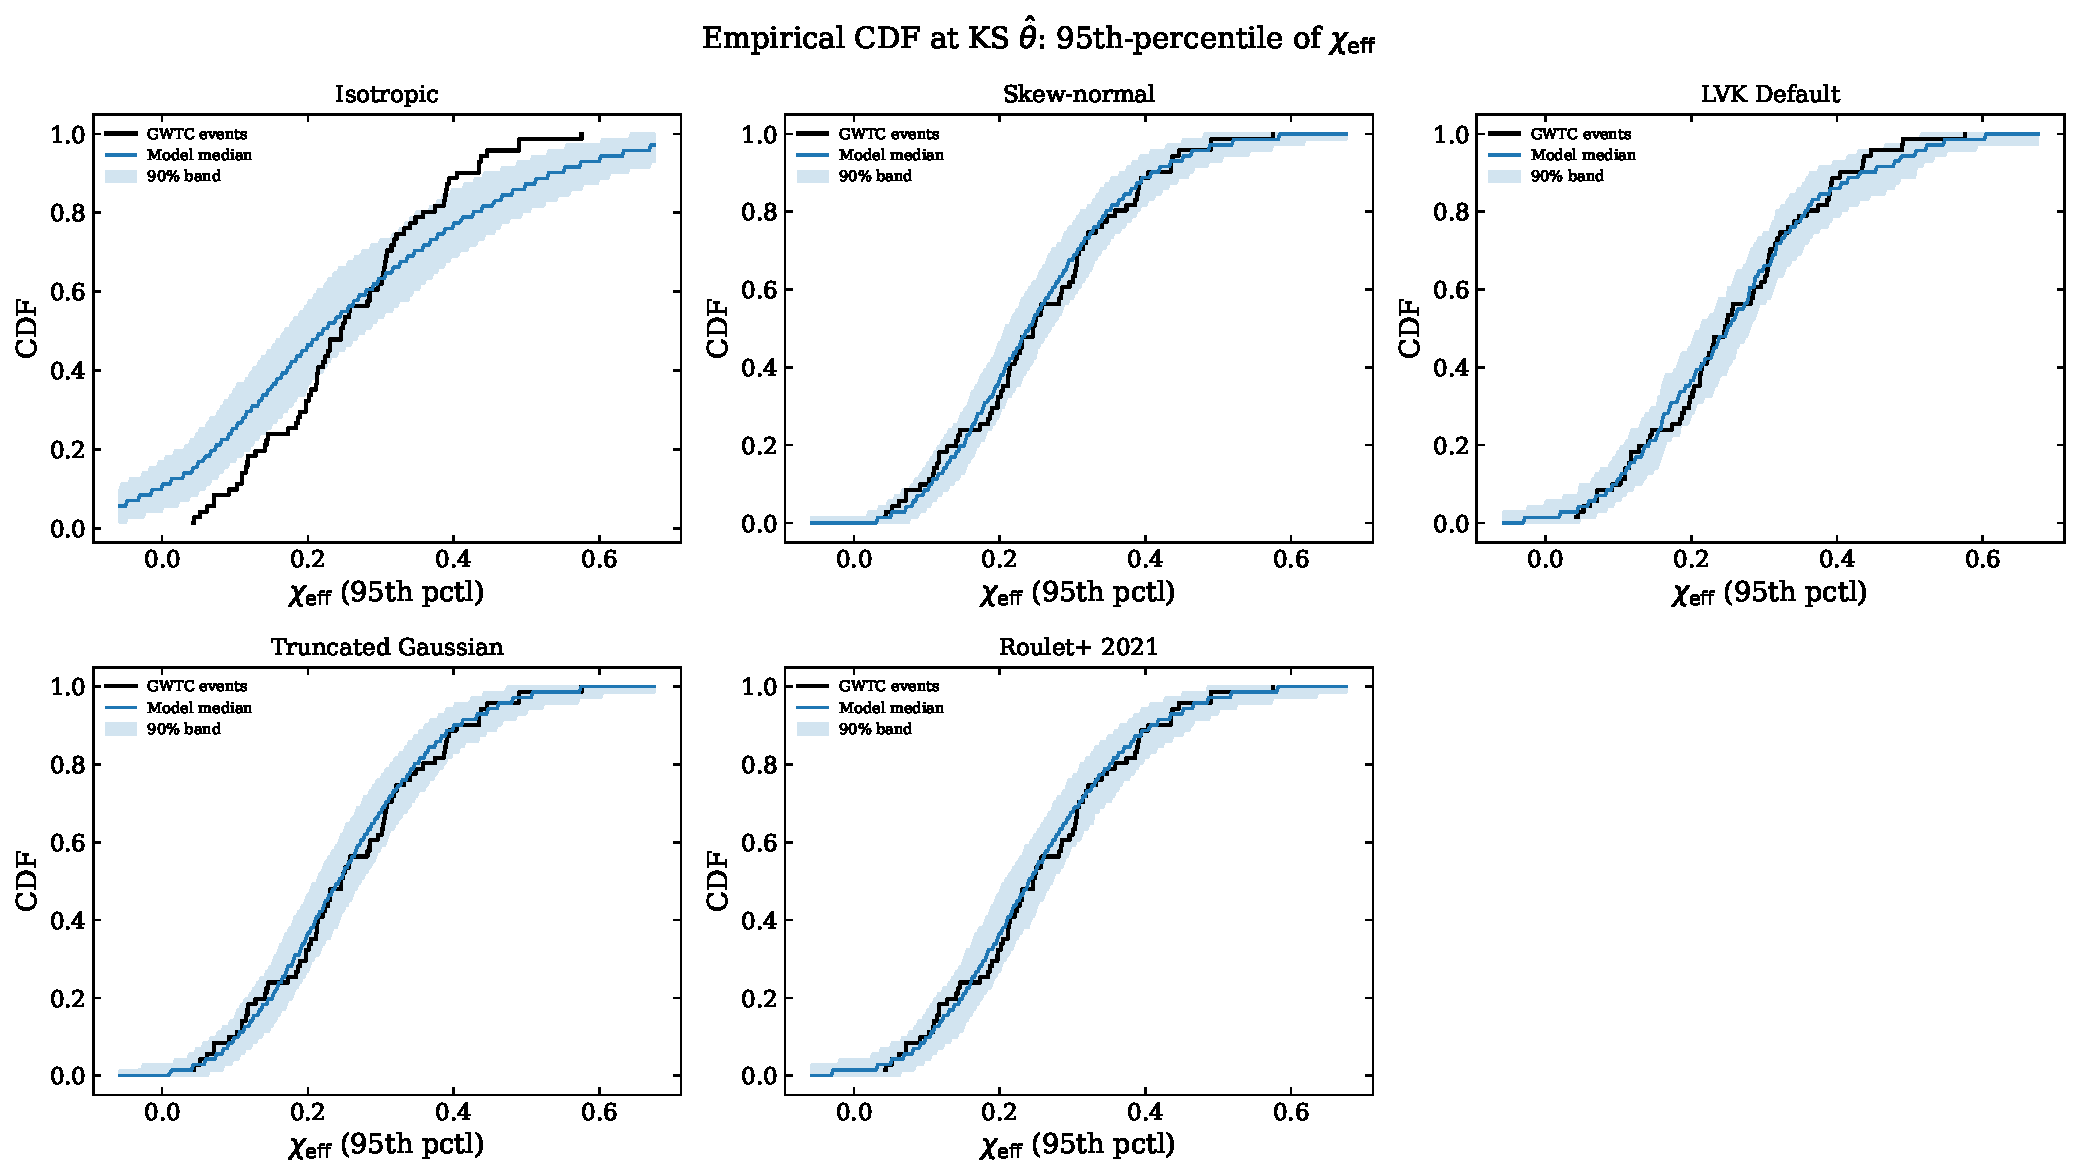
\includegraphics[width=\textwidth]{fig_cdf_95th.pdf}
  \caption{Same as Figure~\ref{fig:cdf5} but for the 95th percentile
           of \chieff.}
  \label{fig:cdf95}
\end{figure}

Table~\ref{tab:ks} summarises the KS-based results.

\begin{table}[htbp]
\centering
\caption{Binning-free goodness-of-fit results using the KS test
statistic~\eqref{eq:ks}. $D_\mathrm{min}$ is the minimised KS distance;
$p$ is the calibrated $p$-value (\Nmock~=~500).  The isotropic model
is rejected at the 5\% level ($p = 0.024$).}
\label{tab:ks}
\begin{tabular}{lccc}
\toprule
Model & $D_\mathrm{min}$ & $p$-value ($\chi^2$) & $p$-value (KS) \\
\midrule
Isotropic          & 0.330 & 0.074 & \textbf{0.024} \\
Skew-normal        & 0.113 & 0.548 & 0.706 \\
LVK Default        & 0.097 & 0.146 & 0.802 \\
Truncated Gaussian & 0.113 & 0.230 & 0.742 \\
Roulet+ 2021       & 0.112 & 0.258 & 0.640 \\
\bottomrule
\end{tabular}
\end{table}

% ══════════════════════════════════════════════════════════════════════════════
\section{Discussion}\label{sec:discussion}

The calibrated $p$-values quantify how well each population model reproduces
the observed distribution of \chieff posterior quantiles.  Models with
$p \lesssim 0.05$ would be disfavoured at the 95\% level.

Key caveats:
\begin{itemize}
  \item The $\chi^2$ test is sensitive to the choice of binning; the
        CDF-based KS test provides a binning-free cross-check.
  \item The effective sample size $N_\mathrm{eff}$ of the re-weighted
        injection set varies across models, affecting the reliability
        of the predicted distributions.
  \item For events with weak \chieff constraints, the PE posterior quantiles
        are dominated by the PE prior rather than the signal, reducing the
        discriminating power of the test.
  \item Free-parameter models benefit from the flexibility of fitting;
        the mock calibration accounts for this look-elsewhere effect.
\end{itemize}

\end{document}
